Одной из поставленных в данном семестре задач стало изучение возможностей многопоточного программирования с использованием программной библиотеки Qt. Программирование потоков осуществляется с помощью класса QThreads, а также механизма сигналов и слотов.

Все это необходимо для того, чтобы реализовать в системе <<COEX>> параллельное выполнение программных модулей (<<плагинов>>), осуществляющих поиск остаточных данных с образа системы, изображений, различных файлов и т.д. 

\subsubsection{ Сигналы и слоты }

Сигналы и слоты используются для связи между объектами. Механизм сигналов и слотов --- это основная особенность Qt и, вероятно, основная часть Qt, которая больше всего отличается по функциональности от других библиотек.

Более старые инструментарии обеспечивают подобную связь с помощью функций обратного вызова. Обратный вызов --- это указатель на функцию. Если необходимо, чтобы функция обработки уведомила о некотором событии, ей передается указатель на другую функцию (отзыв). Функция обработки вызовет функцию обратного вызова, когда это будет уместно. Но данный подход имеет два фундаментальных недостатка: во-первых, он не типобезопасен. Мы некогда не сможем проверить, что функция обработки вызывает отзыв с правильными аргументами. Во-вторых, этот метод жестко связан с функцией обработки, так как она должна знать, какой отзыв вызывать.

В Qt используется техника, альтернативная функциям обратного вызова: механизм сигналов и слотов. Сигнал испускается, когда происходит определенное событие. Слот --- это функция, вызываемая в ответ на определенный сигнал.

Этот механизм типобезопасен: сигнатура сигнала должна соответствовать сигнатуре принимающего слота (фактически, слот может иметь более короткую сигнатуру, чем сигнал, который он получает, поскольку может игнорировать лишние аргументы). Сигналы и слоты связаны нежёстко: класс, испускающий сигналы, не знает и не интересуется, который из слотов получит сигнал. Механизм сигналов и слотов Qt гарантирует, что, если сигнал соединен со слотом, слот будет вызываться с параметрами сигнала в нужный момент. Сигналы и слоты могут иметь любое количество аргументов любых типов. Они полностью типобезопасны.

Все классы, наследуемые от QObject или одного из его подклассов (например, QWidget) могут содержать сигналы и слоты. Сигналы испускаются при изменении объектом своего состояния, если это изменение может быть интересно другим объектам. Все объекты делают это для связи с другими объектами. Их не заботит, получает ли кто-нибудь испускаемые ими сигналы. Это является истинной инкапсуляцией информации, и она гарантирует, что объекты могут использоваться как отдельные компоненты программного обеспечения.

Слоты могут получать сигнал, но они также являются обыкновенными функциями-членами. Также, как объект не знает, получает ли кто-нибудь сигналы, испускаемые им, слоты не знают, существуют ли сигналы, с ними связанные. Это гарантирует, что можно создать полностью независимые Qt-компоненты.

Можно присоединять к одному слоту столько сигналов, сколько необходимо, и один сигнал может быть соединен со столькими слотами, сколько требуется. Также возможно соединение сигнала непосредственно с другим сигналом (второй сигнал будет испускаться немедленно всякий раз, когда испускается первый).

Вместе сигналы и слоты представляют собой мощный механизм компонентного программирования. Графическое представление связи сигналов и слотов различных объектов можно увидеть на рисунке~\ref{signals-slots:signals-slots}. \cite{signalsandslots}

\begin{figure}[h!]
\center{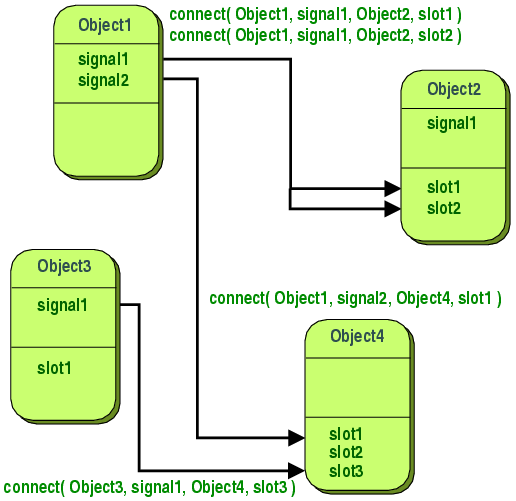
\includegraphics[width=0.8\linewidth]{signals-slots}}
\caption{ Механизм сигналов и слотов для связи объектов в Qt }
\label{signals-slots:signals-slots}
\end{figure}

\subsubsection{ Потоки QThreads }

В многопоточных приложениях, обслуживание интерфейса производится в отдельном потоке, а обработка данных -- в другом (одном или нескольких) потоке. В результате приложение сохраняет возможность откликаться на действия пользователя даже во время интенсивной обработки данных. Еще одно преимущество многопоточности -- на многопроцессорных системах различные потоки могут выполняться на различных процессорах одновременно, что несомненно увеличивает скорость исполнения.

Для реализации потоков Qt предоставляет класс QThread.

Поток — это независимая задача, которая выполняется внутри процесса и разделяет вместе с ним общее адресное пространство, код и глобальные данные.

Процесс, сам по себе, не является исполнительной частью программы, поэтому для исполнения программного кода он должен иметь хотя бы один поток (далее -- основной поток). Конечно, можно создавать и более одного потока. Вновь созданные потоки начинают выполняться сразу же, параллельно с главным потоком, при этом их количество может изменяться — одни создаются, другие завершаются. Завершение основного потока приводит к завершению процесса, независимо от того, существуют другие потоки или нет. Создание нескольких потоков в процессе получило название многопоточность. \cite{threadsandprocesses}

Для использования многопоточности нужно унаследовать класс от QThread. Чтобы запустить поток, нужно вызвать метод start().

Каждый поток может иметь собственный цикл обработки событий. Главный поток начинает цикл обработки событий, используя QCoreApplication::exec(); другие потоки могут начать свои циклы обработки событий, используя QThread::exec().

Цикл обработки событий потока делает возможным использование потоком некоторых неграфических классов Qt, которые требуют наличия цикла обработки событий (такие как QTimer, QTcpSocket и QProcess). Это также даёт возможность соединить сигналы из любых потоков со слотами в определённом потоке (рис.~\ref{thread-cycle:thread-cycle}). \cite{threads}

\begin{figure}[h!]
\center{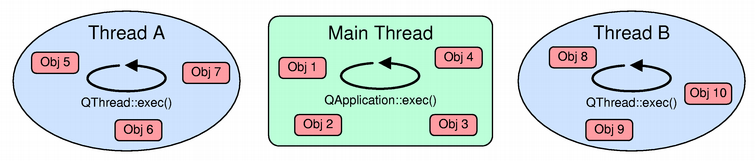
\includegraphics[width=0.8\linewidth]{thread-cycle}}
\caption{ Цикл обработки событий потоков в Qt }
\label{thread-cycle:thread-cycle}
\end{figure}

Для того, чтобы запускать программные модули на выполнение в нескольких потоках и должным образом завершать их выполнение, понадобилось написать контроллер --- объект, который создает потоки для уже существующих объектов (самих плагинов), перемещает эти объекты в созданные потоки. Далее он запускает их выполнение при помощи метода Controller::start\_threads(). После того, как каждый поток завершается, он посылает сигнал контроллеру о завершении finished() и переходит в режим ожидания. Когда все потоки завершаются, контроллер задействует слот stop\_threads(), предназначенный для того, чтобы послать сигнал об успешном завершении работы как всех потоков, так и работы самого контроллера, основной программе. При этом для связи сигналов и слотов используется функция connect(object\_1, SIGNAL(signal\_1), object\_2, SLOT(slot\_2)).  

Поскольку главный поток (основная программа) начинает цикл обработки событий, используя QCoreApplication::exec(), при получении сигнала finished(), сгенерированного контроллером, цикл обработки событий главного потока прерывается и главная программа успешно завершается. 

Алгоритм работы основной программы представлен на рисунке~\ref{main-qthreads:main-qthreads}, контроллера --- на рисунке~\ref{controller-qthreads:controller-qthreads}. 

\begin{figure}[h!]
\center{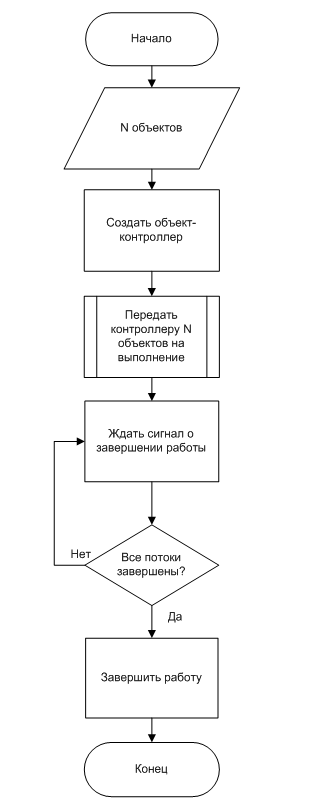
\includegraphics[width=0.5\linewidth]{main-qthreads}}
\caption{ Алгоритм работы основной программы qthreads }
\label{main-qthreads:main-qthreads}
\end{figure}

\clearpage

\begin{figure}[ht]
\center{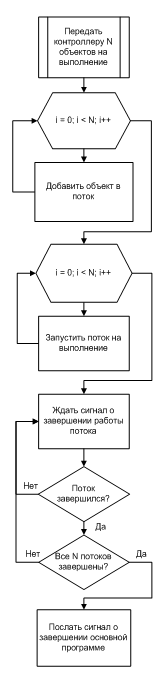
\includegraphics[width=0.3\linewidth]{controller-qthreads}}
\caption{ Алгоритм работы контроллера qthreads }
\label{controller-qthreads:controller-qthreads}
\end{figure}

\clearpage

Результат вывода программы представлен на рисунке~\ref{program-output:program-output}.

\begin{figure}[h!]
\center{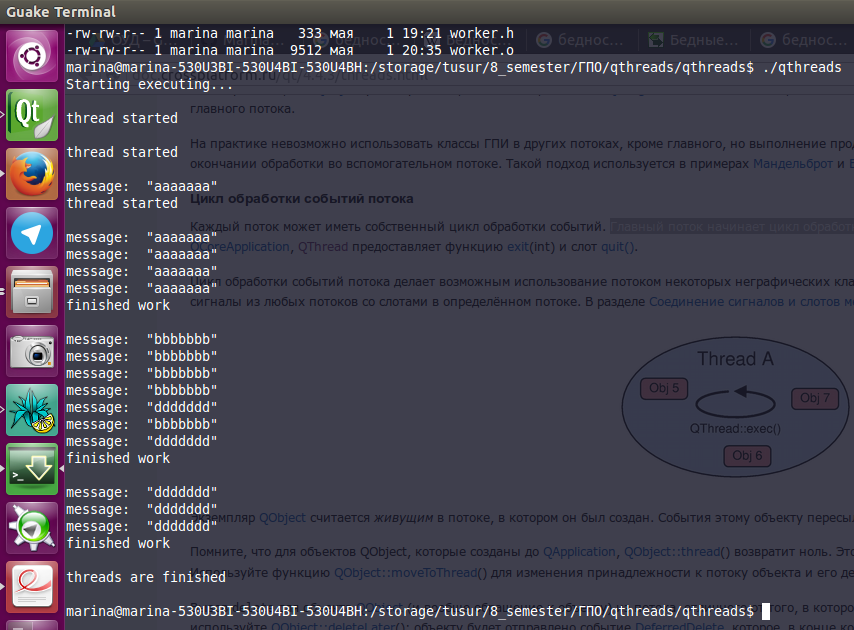
\includegraphics[width=0.8\linewidth]{program-output}}
\caption{ Вывод программы qthreads }
\label{program-output:program-output}
\end{figure}

Кроме написания потокового контроллера был доработан плагин ThreadTaskICQ таким образом, чтобы учитывались особенности работы с механизмом сигналов и слотов. Только после этого плагин может быть запущен в потоке с использованием класса QThreads.  

\clearpage
